\documentclass[11pt,a4paper]{article}
\usepackage[utf8]{inputenc}
\usepackage[T1]{fontenc}
\usepackage{amsthm} %numéroter les questions
\usepackage[frenchb]{babel}
\usepackage{datetime}
\usepackage{xspace} % typographie IN
\usepackage{hyperref}% hyperliens
\usepackage[all]{hypcap} %lien pointe en haut des figures
\usepackage[french]{varioref} %voir x p y
\usepackage{fancyhdr}% en têtes
%\input cyracc.def
\usepackage[]{graphicx} %include pictures
\usepackage{pgfplots}
\usepackage[]{circuitikz}
\usepackage{ifthen}

\usepackage[top=1.3 in, bottom=1.3 in, left=1.3 in, right=1.3 in]{geometry} % Yeah, that's bad to play with margins
\usepackage[]{pdfpages}

\usepackage[]{attachfile}

\usepackage{float}
\usepackage{subfig}

\usepackage{todonotes} % \missingfigure
\usepackage{gensymb} % \ohm

\usepackage{framed}

\newdateformat{mydate}{2016--2017}%hack pour remplacer \THEYEAR


\newboolean{corrige}
\ifx\correction\undefined
\setboolean{corrige}{false}% pas de corrigé
\else
\setboolean{corrige}{true}%corrigé
\fi

%\setboolean{corrige}{false}% pas de corrigé

\newboolean{annexes}
\setboolean{annexes}{true}%annexes
%\setboolean{annexes}{false}% pas de annexes

\definecolor{darkblue}{rgb}{0,0,0.5}

\newboolean{mos}
%\setboolean{mos}{true}%annexes
\setboolean{mos}{false}% pas de annexes

\usepackage{aeguill} %guillemets

%% fancy header & foot
\pagestyle{fancy}
%Numero du TP :
\def \labonumber {Projet -- Partie 3}
\lhead{[ELEC-H-310] Choucroute numérique\\ \labonumber}
\rhead{\mydate\today\\ page \thepage}
\chead{\ifthenelse{\boolean{corrige}}{Corrigé}{}}
\cfoot{}
%%

\pdfinfo{
/Author (Quentin Delhaye, Ken Hasselmann, ULB -- BEAMS)
/Title (\labonumber ELEC-H-310)
/ModDate (D:\pdfdate)
}

\hypersetup{
pdftitle={\labonumber [ELEC-H-310] Choucroute numérique},
pdfauthor={Quentin Delhaye, Ken Hasselmann, ULB -- BEAMS},
pdfsubject={}
}

\theoremstyle{definition}% questions pas en italique
\newtheorem{Q}{Question}[] % numéroter les questions [section] ou non []

\newcommand{\reponse}[1]{% pour intégrer une réponse : \reponse{texte} : sera inclus si \boolean{corrige}
	\ifthenelse {\boolean{corrige}} {\paragraph{Réponse :} \color{darkblue}   #1\color{black}} {}
 }

\newcommand{\addcontentslinenono}[4]{\addtocontents{#1}{\protect\contentsline{#2}{#3}{#4}{}}}

\date{\vspace{-1.7cm}\mydate\today}
\title{\vspace{-2cm}\labonumber\\ Électronique numérique [ELEC-H-310]\\Conception d'une régulation de refroidissement~: \\ interactions avec l'utilisateur\ifthenelse{\boolean{corrige}}{~\\Corrigé}{}}

%\author{\vspace{-1cm}}%\textsc{Yannick Allard}}

\setlength{\parskip}{0.2cm plus2mm minus1mm} %espacement entre §
\setlength{\parindent}{0pt}


















\begin{document}
\pagestyle{empty}
\maketitle
% \vspace*{-1cm}




% ########   ##     ##  ##########  
% ##     ##  ##     ##      ##      
% ##     ##  ##     ##      ##      
% ########   ##     ##      ##      
% ##     ##  ##     ##      ##      
% ##     ##  ##     ##      ##      
% ########    #######       ##      

\section*{But de la manipulation}
Durant trois laboratoires, vous serez amenés à réaliser une mini-climatisation basée sur un ventilateur à hélice.
Il vous sera également demandé de pouvoir interagir localement (clavier) avec le dispositif.

Dans ce troisième et dernier labo, vous serez amenés à ajouter deux modes d’interactions entre votre plateforme de contrôle de la température et l’utilisateur~: soit localement avec un clavier, soit à distance à travers un port série.

Au terme de ce laboratoire, vous devriez avoir terminé votre centrale de climatisation


\section*{Prérequis}
Avant d’entrer au laboratoire, il est demandé de lire le cahier des charges du projet «~Conception d’une régulation de refroidissement~».


\section*{Objectifs}
À la fin de ce laboratoire, vous devez être capables~:
\begin{itemize}
	\item De réaliser une connexion série entre deux processeurs et d'en expliquer le fonctionnement.
	\item De faire communiquer de nombreux périphériques entre eux.
\end{itemize}


\newpage





% ########   ##      ##  ##########  ########     #####    
%    ##      ###     ##      ##      ##     ##  ##     ##  
%    ##      ## ##   ##      ##      ##     ##  ##     ##  
%    ##      ##  ##  ##      ##      ########   ##     ##  
%    ##      ##   ## ##      ##      ##   ##    ##     ##  
%    ##      ##     ###      ##      ##    ##   ##     ##  
% ########   ##      ##      ##      ##     ##    #####    


\section{Introduction}
Durant trois laboratoires, vous serez amenés à réaliser une mini-climatisation basée sur un ventilateur à hélice.
Il vous sera également demandé de pouvoir interagir localement (clavier) avec le dispositif.

Lors de ce laboratoire, vous allez dans un premier temps faire en sorte de pouvoir interagir à travers le clavier de la carte d’extension.
Selon la chaîne de caractères entrés, divers changements seront à prévoir dans le fonctionnement de la carte (ex~: changement de la température de référence, de la période d’échantillonnage, ...).

Par la suite, vous ferez en sorte de pouvoir réaliser ces mêmes changements à distance.
Un PC, connecté au processeur par un câble série, jouera le rôle de la salle de commande vous permettant d’interagir avec un processus sans être physiquement sur place.






%  #######   ##            ###     ##     ##  ########   #########  ########   
% ##     ##  ##           ## ##    ##     ##     ##      ##         ##     ##  
% ##         ##          ##   ##   ##     ##     ##      ##         ##     ##  
% ##         ##         ##     ##  ##     ##     ##      ######     ########   
% ##         ##         #########   ##   ##      ##      ##         ##   ##    
% ##     ##  ##         ##     ##    ## ##       ##      ##         ##    ##   
%  #######   #########  ##     ##     ###     ########   #########  ##     ##  



\section{Interfaçage du clavier}
\begin{figure}[H]
\center
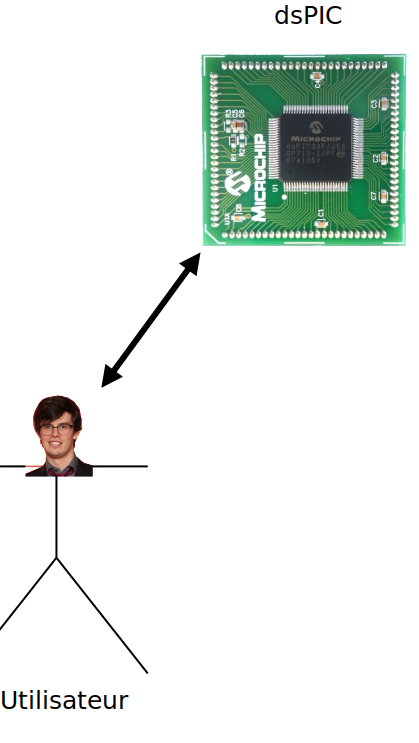
\includegraphics[width=0.3\textwidth]{utilisateur}
\caption{Interaction entre l'utilisateur et la plate-forme.}
\label{fig:user}
\end{figure}

Comme expliqué dans le guide de programmation, le clavier est relié sur des bornes d’I/O génériques du microcontrôleur.
Une fonction permettant de recueillir la touche enfoncée vous sera fournie.

\begin{itemize}
	\item À l’aide du guide de programmation, expliquez le principe général de ce clavier matriciel.
	\item Dans la phase d’initialisation de votre code, configurez correctement les bornes l’entrée/sortie reliées au clavier.
	\item Une fonction permettant de lire la touche enfoncée vous est fournie.
	Si une touche est effectivement enfoncée, elle renvoie le caractère correspondant ( ‘0’ à ‘9’ ou ‘A’ à ‘F’).
	Dans le cas contraire, elle renvoie la valeur ‘z’.
	\item Parcourez le code de cette fonction, et expliquez son fonctionnement.
\end{itemize}

Maintenant que le clavier fonctionne, vous pouvez écrire la fonction permettant de modifier le comportement de votre centrale en fonction des touches enfoncées.
La liste des ordres possibles est donnée dans le cahier des charges global.
\begin{itemize}
	\item La fonction permettant de lire les touches nécessite un grand nombre d’instructions.
	Où faut-il l’appeler afin de ne pas bloquer inutilement le processeur.
	\item Lorsque l’utilisateur est en train de taper sur le clavier, le LCD doit afficher la touche enfoncée.
	Une fois la commande entrée ou annulée, le LCD doit de nouveau afficher la température.
\end{itemize}







%  #######   #########  ########   ########   #########  
% ##     ##  ##         ##     ##     ##      ##         
% ##         ##         ##     ##     ##      ##         
%  #######   ######     ########      ##      ######     
%        ##  ##         ##   ##       ##      ##         
% ##     ##  ##         ##    ##      ##      ##         
%  #######   #########  ##     ##  ########   #########  


\section{Connexion série}
Dans cette partie, vous allez envoyer des données au PC via le port série pour suivre l'évolution de la température, ainsi que recevoir des commandes du PC pour régler la régulation.

Le dernier module à configurer est le port série, permettant de communiquer avec un PC distant.
Ce module porte le nom d’UART (Universal Asynchronous Receiver / Transmitter).
Avant de pouvoir réaliser la communication, vous devrez configurer le dsPIC et le PC afin qu’ils «~parlent le même langage~».
Nous allons commencer par le dsPIC.

\begin{itemize}
	\item À l’aide du guide programmation, configurez l’UART2 de sorte à avoir une communication respectant le format suivant~:
	\begin{itemize}
		% \item Baudrate~: 19200 bits/s
		\item Baudrate~: 9600 bits/s
		\item Bits de données~: 8
		\item Pas de bit de parité
		\item Un seul stop bit
		\item Par de contrôle de flux
	\end{itemize}
	\item Donnez la signification de ces différents paramètres.
\end{itemize}

\subsection{Envoi de données vers le PC}
Pour envoyer des données, référez-vous au code d'exemple \texttt{initUART} et au guide de programmation.
Comme l'indique le cahier des charges, vous devrez envoyer cinq caractères pour chaque mesure de température~: «~42.5\textbackslash n~», où «~\textbackslash n~» est le caractère de retour à la ligne.

Pour afficher les données sur le PC, il vous suffit d'exécuter le script \texttt{graph.py}.



\subsection{Envoi d'une commande depuis le PC}
% \begin{figure}[H]
% \center
% 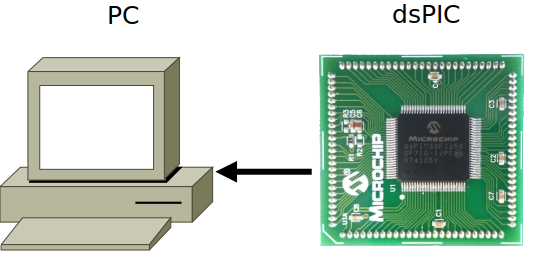
\includegraphics[width=0.4\textwidth]{serie}
% \caption{Connexion série entre la plate-forme et le PC.}
% \label{fig:serie}
% \end{figure}

Coté PC, ouvrez une fenêtre \texttt{putty}, et entrez les mêmes paramètres de format de trame.

% Une fois le protocole de communication établi, il reste à effectivement envoyer les données.
% Commencez par la transmission du dsPIC vers le PC.
% \begin{itemize}
% 	\item Écrivez une fonction permettant d’afficher la température sur l’hyperterminal.
% 	Pour ce faire, vous devrez écrire plusieurs valeurs successives dans le registre d’envoi \texttt{U2TXREG}, en prenant à chaque fois soin de vérifier que le buffer n’est pas plein afin de ne pas écraser les caractères qui n’auraient pas été envoyés.
% 	\item Modifiez votre programme de sorte à exécuter cette fonction toutes les 1~s.
% \end{itemize}

Enfin, il ne reste plus qu’à configurer le $\mu$C pour qu’il puisse accepter des commandes en provenance du port série.
\begin{itemize}
	\item Écrivez une routine permettant de lire le dernier caractère reçu.
	Justifiez pourquoi cette routine doit être appelée sous forme d’interruption.
	\item Vérifiez que votre $\mu$C est bien capable de recevoir un caractère entré sur le PC.
	\item Complétez votre routine de manière à répondre aux ordres décrits dans le cahier des charges global.
\end{itemize}






%  #######   ##     ##   #######   ##########    #####    ##       ##  
% ##     ##  ##     ##  ##     ##      ##      ##     ##  ###     ###  
% ##         ##     ##  ##             ##      ##     ##  ## ## ## ##  
% ##         ##     ##   #######       ##      ##     ##  ##  ###  ##  
% ##         ##     ##         ##      ##      ##     ##  ##       ##  
% ##     ##  ##     ##  ##     ##      ##      ##     ##  ##       ##  
%  #######    #######    #######       ##        #####    ##       ##  



\section{Personnalisatrion du projet}
Votre centrale est maitnenant fonctionnelle, vous pouvez lui ajouter différentes fonctionnalités afin de l'améliorer.


\end{document}
